\ffigbox[\FBwidth]{%
\caption{\centering Graphe de poissons}\label{Fig:td_5_ex_1_1}
}{
    \fbox{
        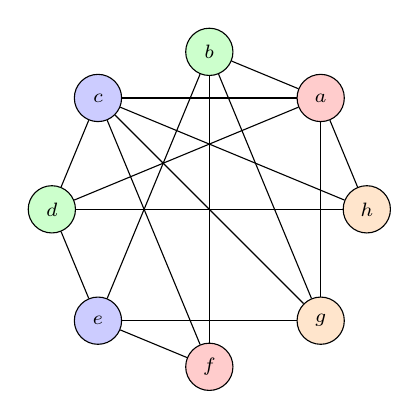
\begin{tikzpicture}[scale=1, 
            main node/.style={circle, draw, fill=blue!20, inner sep=1pt, font=\scriptsize, minimum size=6mm}, 
            cola node/.style={circle, draw, fill=red!20, inner sep=1pt, font=\scriptsize, minimum size=6mm}, 
            colb node/.style={circle, draw, fill=green!20, inner sep=1pt, font=\scriptsize, minimum size=6mm}, 
            colc node/.style={circle, draw, fill=blue!20, inner sep=1pt, font=\scriptsize, minimum size=6mm}, 
            cold node/.style={circle, draw, fill=orange!20, inner sep=1pt, font=\scriptsize, minimum size=6mm}]
            % le cercle de départ 
            % \draw (0, 0) circle [radius=2];
            
            % les sommets initiaux
            \node[cola node] (a) at (45:2)  {\(a\)};
            \node[colb node] (b) at (90:2)  {\(b\)};
            \node[colc node] (c) at (135:2) {\(c\)};
            \node[colb node] (d) at (180:2){\(d\)};
            \node[colc node] (e) at (225:2){\(e\)};
            \node[cola node] (f) at (270:2){\(f\)};
            \node[cold node] (g) at (315:2){\(g\)};
            \node[cold node] (h) at (0:2){\(h\)};
            % ahcd
            \draw (a) -- (b);
            \draw (a) -- (c);
            \draw (a) -- (d);
            \draw (a) -- (g);
            \draw (a) -- (h);

            \draw (b) -- (e);
            \draw (b) -- (f);
            \draw (b) -- (g);

            \draw (c) -- (d);
            \draw (c) -- (f);
            \draw (c) -- (g);
            \draw (c) -- (h);

            \draw (d) -- (e);
            \draw (d) -- (h);

            \draw (e) -- (f);
            \draw (e) -- (g);
        \end{tikzpicture}
    }
}